\documentclass{standalone}
\usepackage{tikz}
\usepackage{amsmath}

\begin{document}

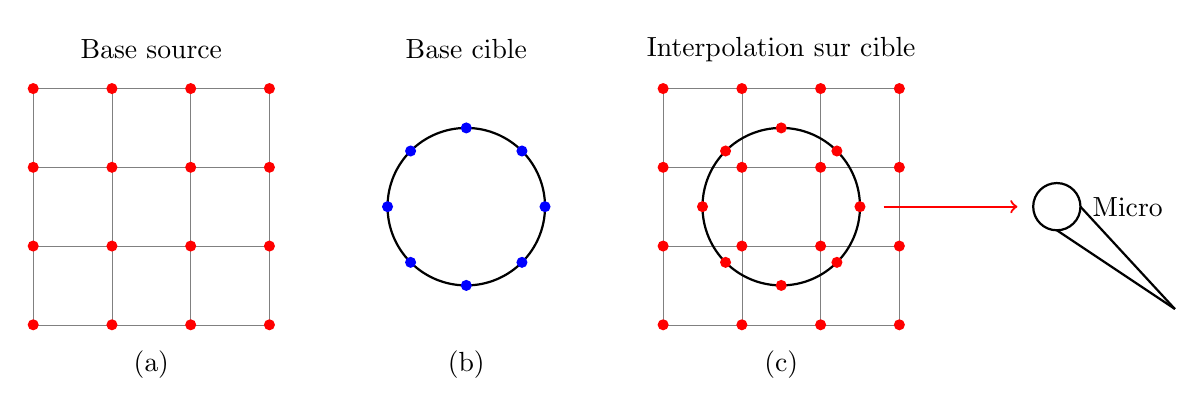
\begin{tikzpicture}

    % Step 1: Base source (rectangular grid)
    \draw[step=1cm,gray,very thin] (-3,0) grid (0,3);
    \node at (-1.5, 3.5) {Base source};
    \node at (-1.5, -0.5) {(a)};
    
    % Adding nodes and elements
    \foreach \x in {-3, -2, -1, 0} {
        \foreach \y in {0, 1, 2, 3} {
            \fill[red] (\x,\y) circle (2pt);
        }
    }
    
    %\node[anchor=west] at (0.2, 1.5) {$\sin(\text{pression})$};
    
    % Step 2: Base cible (circle)
    \draw[thick] (2.5,1.5) circle (1cm);
    \node at (2.5, 3.5) {Base cible};
    \node at (2.5, -0.5) {(b)};
    %\draw[->,thick,red] (2.5,1.5) -- (4, 1.5) node[midway,above] {Interpolation};

    % Discretize the circle with red points
    \foreach \angle in {0,45,...,315} {
        \fill[blue] ({2.5 + 1*cos(\angle)},{1.5 + 1*sin(\angle)}) circle (2pt);
    }
    
    % Step 3: Interpolated solution (target surface)
    \draw[step=1cm,gray,very thin] (5,0) grid (8,3);
    \draw[thick] (6.5,1.5) circle (1cm);
    \node at (6.5, 3.5) {Interpolation sur cible};

    \foreach \angle in {0,45,...,315} {
        \fill[red] ({6.5 + 1*cos(\angle)},{1.5 + 1*sin(\angle)}) circle (2pt);
    }

    \node at (6.5, -0.5) {(c)};
    
    % Step 4: Application of FWH equations
    %\draw[->,thick,red] (8.5,1.5) -- (10, 1.5) node[midway,above] {FWH};
    %\node at (11.5, 1.5) {Calcul du son à distance};
    
    % Additional nodes and elements for interpolated solution
    \foreach \x in {5,6,7,8} {
        \foreach \y in {0,1,2,3} {
            \fill[red] (\x,\y) circle (2pt);
        }
    }

    % Step 4: Application of FWH equations and the microphone
    \node at (10.9, 1.5) {Micro};
    \draw[thick] (10,1.5) circle (0.3cm); % Micro symbol
    \draw[thick] (10.3,1.5) -- (11.5,0.2); % Micro "handle"
    \draw[thick] (10.0,1.2) -- (11.5,0.2); % Micro "handle"
    \draw[->,thick,red] (7.8,1.5) -- (9.5, 1.5); % Arrow from circle to microphone

\end{tikzpicture}

\end{document}